              %******************************************%
              %                                          %
              %     Modello di articolo scientifico      %
              %            di Lorenzo Pantieri �         %
              %                                          %
              %         versione: 26 agosto 2012         %
              %                                          %
              %******************************************%
       

% I seguenti commenti speciali impostano:
% 1. utf8 come codifica di input,
% 2. PDFLaTeX come motore di composizione;
% 3. Articolo.tex come documento principale;
% 4. il controllo ortografico italiano per l'editor.

% !TEX encoding = UTF-8
% !TEX TS-program = pdflatex
% !TEX root = Articolo.tex
% !TEX spellcheck = en-EN

\documentclass[12pt,%                       % corpo del font principale
               a4paper,%                    % carta A4
               oneside,%                    % solo fronte
%              twoside,%                    % fronte-retro
               ]{article}                  % classe report di KOMA-Script;
         
\usepackage{helvet}
\renewcommand*\familydefault{\sfdefault} 	   
\usepackage[T1]{fontenc}                    % codifica dei font:
                                            % NOTA BENE! richiede una distribuzione *completa* di LaTeX,
                                            % per esempio TeXLive o MiKTeX *complete*

\usepackage[utf8]{inputenc}                 % codifica di input; anche [latin1] va bene
                                            % NOTA BENE! va accordata con le preferenze dell'editor

\usepackage[english,italian]{babel}         % per scrivere in italiano e in inglese;
                                            % l'ultima lingua (l'italiano) risulta predefinita

%\usepackage[binding=20mm]{layaureo}          % margini ottimizzati per l'A4;
% rilegatura di 5 mm
\usepackage[a4paper,margin=2cm,footskip=2cm]{geometry}



\usepackage{indentfirst}                    % rientra il primo capoverso di ogni sezione

\usepackage{booktabs}                       % tabelle

\usepackage{tabularx}                       % tabelle di larghezza prefissata

\usepackage{graphicx}                       % immagini

\usepackage{subfig}                         % sottofigure, sottotabelle

\usepackage{caption}                        % didascalie

\usepackage{listings}                       % codici

\usepackage[font=small]{quoting}            % citazioni

\usepackage{amsmath,amssymb,amsthm}         % matematica

\usepackage[italian]{varioref}              % riferimenti completi della pagina

% \usepackage{mparhack,fixltx2e,relsize}      % finezze tipografiche

\usepackage[style=numeric-comp,hyperref,backref,backend=bibtex]{biblatex}	
                                            % eccellente pacchetto per la bibliografia;
                                            % produce uno stile di citazione autore-anno; 
                                            % lo stile "numeric-comp" produce riferimenti numerici
                                          
\bibliography{Bibliografia}                 % database di biblatex 
                                          
\usepackage[dvipsnames]{xcolor}             % colori

\usepackage{lipsum}                         % testo fittizio

\usepackage{eurosym}                        % simbolo dell'euro

\usepackage{hyperref}                       % collegamenti ipertestuali

%\usepackage{bookmark}                       % segnalibri

%*********************************************************************************
% impostazioni-articolo.tex
% di Lorenzo Pantieri (2012)
% file che contiene le impostazioni dell'articolo
%*********************************************************************************


%*********************************************************************************
% Comandi personali
%*******************************************************
%\newcommand{\myName}{Lorenzo Pantieri}                            % autore
\newcommand{\myTitle}{Characterization of Particle Based Simulation Parameters
by means of Artificial Neural Networks}  % titolo
\date{}                                                           % nessuna data

%\title{\myTitle}
%\author{\myName}



%*********************************************************************************
% Impostazioni di amsmath, amssymb, amsthm
%*********************************************************************************

% comandi per gli insiemi numerici (serve il pacchetto amssymb)
\newcommand{\numberset}{\mathbb} 
\newcommand{\N}{\numberset{N}} 
\newcommand{\R}{\numberset{R}} 

% un ambiente per i sistemi
\newenvironment{sistema}%
  {\left\lbrace\begin{array}{@{}l@{}}}%
  {\end{array}\right.}

% definizioni (serve il pacchetto amsthm)
\theoremstyle{definition} 
\newtheorem{definizione}{Definizione}

% teoremi, leggi e decreti (serve il pacchetto amsthm)
\theoremstyle{plain} 
\newtheorem{teorema}{Teorema}
\newtheorem{legge}{Legge}
\newtheorem{decreto}[legge]{Decreto}
\newtheorem{murphy}{Murphy}[section]



%*********************************************************************************
% Impostazioni di biblatex
%*********************************************************************************
\defbibheading{bibliography}{%
\phantomsection
\addcontentsline{toc}{section}{\refname}
\section*{\bibname\markboth{\MakeUppercase{\refname}}{\MakeUppercase{\refname}}}}



%*********************************************************************************
% Impostazioni di listings
%*********************************************************************************
\lstset{language=[LaTeX]Tex,%C++,
    keywordstyle=\color{RoyalBlue},%\bfseries,
    basicstyle=\small\ttfamily,
    %identifierstyle=\color{NavyBlue},
    commentstyle=\color{Green}\ttfamily,
    stringstyle=\rmfamily,
    numbers=none,%left,%
    numberstyle=\scriptsize,%\tiny
    stepnumber=5,
    numbersep=8pt,
    showstringspaces=false,
    breaklines=true,
    frameround=ftff,
    frame=single
} 



%*********************************************************************************
% Impostazioni di hyperref
%*********************************************************************************
% \hypersetup{%
%     hyperfootnotes=false,pdfpagelabels,
%     %draft,	% = elimina tutti i link (utile per stampe in bianco e nero)
%     colorlinks=true, linktocpage=true, pdfstartpage=1, pdfstartview=FitV,%
%     % decommenta la riga seguente per avere link in nero (per esempio per la stampa in bianco e nero)
%     %colorlinks=false, linktocpage=false, pdfborder={0 0 0}, pdfstartpage=1, pdfstartview=FitV,% 
%     breaklinks=true, pdfpagemode=UseNone, pageanchor=true, pdfpagemode=UseOutlines,%
%     plainpages=false, bookmarksnumbered, bookmarksopen=true, bookmarksopenlevel=1,%
%     hypertexnames=true, pdfhighlight=/O,%nesting=true,%frenchlinks,%
%     urlcolor=webbrown, linkcolor=RoyalBlue, citecolor=webgreen, %pagecolor=RoyalBlue,%
%     %urlcolor=Black, linkcolor=Black, citecolor=Black, %pagecolor=Black,%
%     pdftitle={\myTitle},%
%     pdfauthor={\textcopyright\ \myName},%
%     pdfsubject={},%
%     pdfkeywords={},%
%     pdfcreator={pdfLaTeX},%
%     pdfproducer={LaTeX with hyperref and ClassicThesis}%
% }



%*********************************************************************************
% Impostazioni di graphicx
%*********************************************************************************
%\graphicspath{{Immagini/}} % cartella dove sono riposte le immagini



%*********************************************************************************
% Impostazioni di xcolor
%*********************************************************************************
\definecolor{webgreen}{rgb}{0,.5,0}
\definecolor{webbrown}{rgb}{.6,0,0}



%*********************************************************************************
% Impostazioni di caption
%*********************************************************************************
\captionsetup{tableposition=top,figureposition=bottom,font=small,format=hang,labelfont=bf}



%*********************************************************************************
% Altro
%*********************************************************************************

% [...] ;-)
\newcommand{\omissis}{[\dots\negthinspace]}

% eccezioni all'algoritmo di sillabazione
\hyphenation{Fortran ma-cro-istru-zio-ne nitro-idrossil-amminico}

\pagenumbering{gobble} %to switch off page numbering.               % file con le impostazioni personali

\begin{document}
%\pagestyle{headings} 
%******************************************************************
% Materiale iniziale
%******************************************************************
% !TEX encoding = UTF-8
% !TEX TS-program = pdflatex
% !TEX root = ../Articolo.tex
% !TEX spellcheck = it-IT

%*******************************************************
% Frontespizio
%*******************************************************
\begin{titlepage}
\pdfbookmark{Frontespizio}{Frontespizio}
\changetext{}{}{}{((\paperwidth - \textwidth) / 2) - \oddsidemargin - \hoffset - 1in}{}

\begin{center}


% Upper part of the page

\includegraphics[width=0.3\textwidth]{045PFM_Logo_Original}\\[1cm]    

\textsc{\LARGE \myDepartment}\\[1.5cm]


% This document uses the following counting scheme
%    I   - Year for Q1 of the year Year
%    II  - Year ...
%    III - Year
%    IV  - Year
\textsc{\Large \myTitle ~ - \RM{8}  - 2015}\\[0.5cm]


% Title
\HRule \\[0.4cm]
{ \huge \bfseries \myPhd}\\[0.4cm]

\HRule \\[1.5cm]

% Author and supervisor

\begin{minipage}{0.8\textwidth}
\begin{center} \large

\emph{Author:}\\[0.4cm]

%irstname \textsc{Lastname}
\myName \\
\texttt{\myemail}\\[1.5cm]

\emph{Supervisors:} \\[0.4cm]

\myProf \\[0.2cm]
\myOtherProf \\ [0.2cm]
%\end{flushright}

\end{center}

\end{minipage}

\vfill

% Print the current date at the bottom of the page
{\large \myTime}

\end{center}

\end{titlepage}

%% !TEX encoding = UTF-8
% !TEX TS-program = pdflatex
% !TEX root = ../Articolo.tex
% !TEX spellcheck = it-IT

%*******************************************************
% Indici
%*******************************************************
\pdfbookmark{\contentsname}{tableofcontents}
\setcounter{tocdepth}{2}
\tableofcontents
\markboth{\contentsname}{\contentsname} 

%*******************************************************
% Elenco delle figure
%*******************************************************    
\phantomsection
\pdfbookmark{\listfigurename}{lof}
\listoffigures

%*******************************************************
% Elenco delle tabelle
%*******************************************************
\phantomsection
\pdfbookmark{\listtablename}{lot}
\listoftables
       
	   
\newpage
% !TEX encoding = UTF-8
% !TEX TS-program = pdflatex
% !TEX root = ../Articolo.tex
% !TEX spellcheck = it-IT

%*******************************************************
% Sommario+Abstract
%*******************************************************
\phantomsection
\pdfbookmark{Sommario}{Sommario}
\section*{Sommario}

\lipsum[1]

\selectlanguage{english}
\pdfbookmark{Abstract}{Abstract}
\section*{Abstract}

\lipsum[2]

\selectlanguage{italian}


%******************************************************************
% Materiale principale
%******************************************************************
% !TEX encoding = UTF-8
% !TEX TS-program = pdflatex
% !TEX root = ../Articolo.tex
% !TEX spellcheck = it-IT

%************************************************
\section{Lorem}
\label{sec:lorem}
%************************************************

Lorem ipsum dolor sit amet, consectetuer adipiscing elit. Ut purus elit, vestibulum ut, placerat ac, adipiscing vitae, felis. Curabitur dictum gravida mauris. Nam arcu libero, nonummy eget, consectetuer id, vulputate a, magna. Donec vehicula augue eu neque.

\subsection{Esempi}

\subsubsection{Tabelle}

\lipsum

\begin{table}[tb]
\caption[Un esempio di tabella mobile]{Un esempio di tabella mobile.}
\label{tab:esempio}
\centering
\begin{tabular}{cc}
\toprule
$p$ & $\lnot p$ \\ 
\midrule
V   & F \\ 
F   & V \\
\bottomrule 
\end{tabular}
\end{table}

La tabella~\vref{tab:esempio} fornisce un esempio di tabella mobile.

\lipsum[1-2]


\subsubsection{Figure}

\lipsum[2]

\begin{figure}[tb] 
\centering 
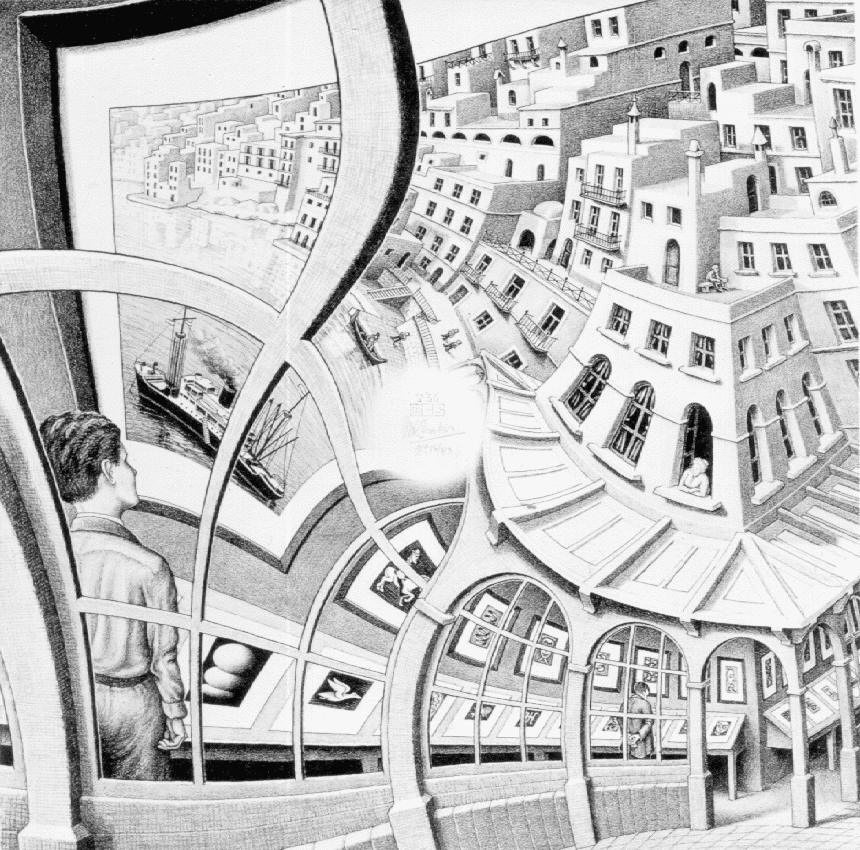
\includegraphics[width=0.5\columnwidth]{GalleriaStampe} 
\caption[Un esempio di figura mobile]{Un esempio di figura mobile (l'immagine, che riproduce la litografia \emph{Galleria di stampe}, di M.~Escher,\index{Escher, M.~C.} proviene da \url{http://www.mcescher.com/}).}
\label{fig:galleria} 
\end{figure}

La figura~\vref{fig:galleria} fornisce un esempio di figura mobile.

\lipsum[3]

\begin{figure}[tb]
\centering
\subfloat[Asia personas duo.]
{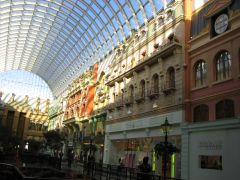
\includegraphics[width=.45\columnwidth]{Lorem}} \quad
\subfloat[Pan ma signo.]
{\label{fig:ipsum}%
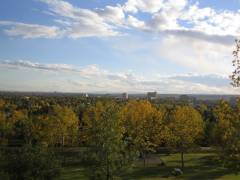
\includegraphics[width=.45\columnwidth]{Ipsum}} \\
\subfloat[Methodicamente o uno.]
{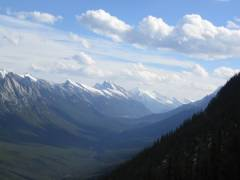
\includegraphics[width=.45\columnwidth]{Dolor}} \quad
\subfloat[Titulo debitas.]
{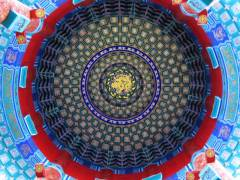
\includegraphics[width=.45\columnwidth]{Sit}}
\caption[Tu duo titulo debitas latente]{Tu duo titulo debitas
latente.}
\label{fig:esempio}
\end{figure}

La figura~\vref{fig:esempio} costituisce un esempio di figura mobile.

\lipsum[4]

% !TEX encoding = UTF-8
% !TEX TS-program = pdflatex
% !TEX root = ../Articolo.tex
% !TEX spellcheck = it-IT

%************************************************
\section{Ipsum}
\label{sec:ipsum}
%************************************************


Lorem ipsum dolor sit amet, consectetuer adipiscing elit. Nam dui ligula, fringilla a, euismod sodales, sollicitudin vel, wisi. Morbi auctor lorem non justo. Nam lacus libero, pretium at, lobortis vitae, ultricies et, tellus.
\begin{description}
\item[Lorem ipsum dolor] sit amet, consectetuer adipiscing elit. Ut purus elit, vestibulum ut, placerat ac $\lim_{n \to \infty}\sum_{k=1}^n \frac{1}{k^2}= \frac{\pi^2}{6}$.
\item[Mauris ut leo.]
Cras viverra metus rhoncus sem. Nulla et lectus vestibulum urna fringilla ultrices. Phasellus eu tellus sit amet tortor gravida placerat.
\[
\lim_{n \to \infty}\sum_{k=1}^n \frac{1}{k^2}= \frac{\pi^2}{6}.
\]
\end{description}

Nulla malesuada porttitor diam. Donec felis erat, congue non, volutpat at, tincidunt tristique, libero. Vivamus viverra fermentum felis.
\begin{equation}
\label{eq:euler}
e^{i\pi}+1=0.
\end{equation}
Dalla formula~\eqref{eq:euler} 
si deduce che\dots






\subsection{Nozioni basilari}

\subsubsection{Insiemi numerici}

Donec nonummy pellentesque ante. Phasellus adipiscing semper elit.
\begin{equation}
x^2 \geq 0 \quad
\forall x \in \mathbb{R}.
\end{equation}


\subsubsection{Le matrici}

\lipsum[2]
\begin{equation}
A=
\begin{bmatrix}
x_{11} & x_{12} & \dots \\
x_{21} & x_{22} & \dots \\
\vdots & \vdots & \ddots
\end{bmatrix}
\end{equation}



\subsection{Formule fuori corpo}

Proin fermentum massa ac quam. Sed diam turpis, molestie vitae, placerat a, molestie nec, leo. Maecenas lacinia. Nam ipsum ligula, eleifend at, accumsan nec, suscipit a, ipsum. 


\subsubsection{Una formula spezzata con allineamento}

\lipsum[2]
\begin{equation} 
\begin{split} 
a &= b+c-d \\ 
  &= e-f \\ 
  &= g+h \\ 
  &= i. 
\end{split} 
\end{equation}

 
\subsubsection{Casi}

\lipsum[3]
\begin{equation}
f(n):=
\begin{cases} 
2n+1, & \text{con $n$ dispari,} \\ 
n/2,  & \text{con $n$ pari.} 
\end{cases} 
\end{equation}



\subsection{Enunciati e dimostrazioni}

Nunc eleifend consequat lorem. Sed lacinia nulla vitae enim. Pellentesque tincidunt purus vel magna. Integer non enim. Praesent euismod nunc eu purus.
\begin{definizione}[di Gauss] 
Un \emph{matematico} trova ovvio che
$\int_{-\infty}^{+\infty}
e^{-x^2}\,dx=\sqrt{\pi}$. 
\end{definizione} 
\begin{teorema} 
I matematici, se ce ne sono, sono molto rari.
\end{teorema} 

\lipsum[2]

\begin{teorema}[di Pitagora]
La somma dei quadrati costruiti sui cateti uguaglia il quadrato costruito sull'ipotenusa.
\end{teorema}
La dimostrazione viene lasciata per esercizio.

Donec bibendum quam in tellus. Nullam cursus pulvinar lectus. Donec et mi. Nam vulputate metus eu enim. Vestibulum pellentesque felis eu massa.
\begin{teorema}[Sorpresa]
Si ha che $\log(-1)^2=2\log(-1)$.
\end{teorema} 
\begin{proof} 
Si ha che $\log(1)^2 = 2\log(1)$.
Ma si ha anche che $\log(-1)^2=\log(1)=0$.
Quindi $2\log(-1)=0$, da cui la tesi.
\end{proof}
Viene un quadratino a fine dimostrazione.
\begin{legge}
\label{lex:capo}
Il capo ha ragione.
\end{legge}
\begin{decreto}[Aggiornamento alla legge~\ref{lex:capo}]
Il capo ha \emph{sempre} ragione.
\end{decreto}
\begin{legge}
Se il capo ha torto, vedere la 
legge~\ref{lex:capo}.
\end{legge}


Nam dui ligula, fringilla a, euismod sodales, sollicitudin vel, wisi. Morbi auctor lorem non justo. Nam lacus libero, pretium at, lobortis vitae, ultricies et, tellus.
\begin{murphy}
Cras nec ante. Pellentesque a nulla. Cum sociis natoque penatibus et magnis dis parturient montes, nascetur ridiculus mus. Aliquam tincidunt urna.
\end{murphy}

\appendix
% !TEX encoding = UTF-8
% !TEX TS-program = pdflatex
% !TEX root = ../Articolo.tex
% !TEX spellcheck = it-IT

%************************************************
\section{Dolor}
\label{sec:dolor}
%************************************************

\lipsum[1]

\subsection{Mane}
\lipsum[2]

\subsection{Tekel}
\lipsum[3]

\subsection{Fares}
\lipsum[4-5]

% *****************************************************************
% Materiale finale
%******************************************************************
% !TEX encoding = UTF-8
% !TEX TS-program = pdflatex
% !TEX root = ../Articolo.tex
% !TEX spellcheck = it-IT

%*******************************************************
% Bibliografia
%*******************************************************
%\nocite{*}
\printbibliography
\end{document}